\documentclass{article}\usepackage[]{graphicx}\usepackage[]{color}
%% maxwidth is the original width if it is less than linewidth
%% otherwise use linewidth (to make sure the graphics do not exceed the margin)
\makeatletter
\def\maxwidth{ %
  \ifdim\Gin@nat@width>\linewidth
    \linewidth
  \else
    \Gin@nat@width
  \fi
}
\makeatother

\definecolor{fgcolor}{rgb}{0.345, 0.345, 0.345}
\newcommand{\hlnum}[1]{\textcolor[rgb]{0.686,0.059,0.569}{#1}}%
\newcommand{\hlstr}[1]{\textcolor[rgb]{0.192,0.494,0.8}{#1}}%
\newcommand{\hlcom}[1]{\textcolor[rgb]{0.678,0.584,0.686}{\textit{#1}}}%
\newcommand{\hlopt}[1]{\textcolor[rgb]{0,0,0}{#1}}%
\newcommand{\hlstd}[1]{\textcolor[rgb]{0.345,0.345,0.345}{#1}}%
\newcommand{\hlkwa}[1]{\textcolor[rgb]{0.161,0.373,0.58}{\textbf{#1}}}%
\newcommand{\hlkwb}[1]{\textcolor[rgb]{0.69,0.353,0.396}{#1}}%
\newcommand{\hlkwc}[1]{\textcolor[rgb]{0.333,0.667,0.333}{#1}}%
\newcommand{\hlkwd}[1]{\textcolor[rgb]{0.737,0.353,0.396}{\textbf{#1}}}%

\usepackage{framed}
\makeatletter
\newenvironment{kframe}{%
 \def\at@end@of@kframe{}%
 \ifinner\ifhmode%
  \def\at@end@of@kframe{\end{minipage}}%
  \begin{minipage}{\columnwidth}%
 \fi\fi%
 \def\FrameCommand##1{\hskip\@totalleftmargin \hskip-\fboxsep
 \colorbox{shadecolor}{##1}\hskip-\fboxsep
     % There is no \\@totalrightmargin, so:
     \hskip-\linewidth \hskip-\@totalleftmargin \hskip\columnwidth}%
 \MakeFramed {\advance\hsize-\width
   \@totalleftmargin\z@ \linewidth\hsize
   \@setminipage}}%
 {\par\unskip\endMakeFramed%
 \at@end@of@kframe}
\makeatother

\definecolor{shadecolor}{rgb}{.97, .97, .97}
\definecolor{messagecolor}{rgb}{0, 0, 0}
\definecolor{warningcolor}{rgb}{1, 0, 1}
\definecolor{errorcolor}{rgb}{1, 0, 0}
\newenvironment{knitrout}{}{} % an empty environment to be redefined in TeX

\usepackage{alltt}
\usepackage[sc]{mathpazo}
\usepackage[T1]{fontenc}
\usepackage{geometry}
\geometry{verbose,tmargin=2.5cm,bmargin=2.5cm,lmargin=2.5cm,rmargin=2.5cm}
\setcounter{secnumdepth}{2}
\setcounter{tocdepth}{2}
\usepackage{url}
\usepackage[unicode=true,pdfusetitle,
 bookmarks=true,bookmarksnumbered=true,bookmarksopen=true,bookmarksopenlevel=2,
 breaklinks=false,pdfborder={0 0 1},backref=false,colorlinks=false]
 {hyperref}
\hypersetup{
 pdfstartview={XYZ null null 1}}
\usepackage{breakurl}
\IfFileExists{upquote.sty}{\usepackage{upquote}}{}
\begin{document}



\section*{Problem Two Repeat Again}
This model has a better fit using knn and linear model, which is what we had expected since we don't have oscillating function here. We can easily interpret a trend of data so that the fit would be more accurate. It is demonstrated by our code below that a large portion of EPE comes from variance, from some perspective,  it reflects that we have pretty good fit for the data.

\begin{knitrout}
\definecolor{shadecolor}{rgb}{0.969, 0.969, 0.969}\color{fgcolor}\begin{kframe}
\begin{alltt}
\hlkwd{set.seed}\hlstd{(}\hlnum{25041}\hlstd{)}
\hlkwd{par}\hlstd{(}\hlkwc{mfcol} \hlstd{=} \hlkwd{c}\hlstd{(}\hlnum{2}\hlstd{,} \hlnum{2}\hlstd{))}
\hlkwd{require}\hlstd{(FNN)}
\end{alltt}


{\ttfamily\noindent\itshape\color{messagecolor}{\#\# Loading required package: FNN}}

{\ttfamily\noindent\color{warningcolor}{\#\# Warning: package 'FNN' was built under R version 3.0.2}}\begin{alltt}
\hlkwd{require}\hlstd{(fields)}
\end{alltt}


{\ttfamily\noindent\itshape\color{messagecolor}{\#\# Loading required package: fields\\\#\# Loading required package: spam\\\#\# Loading required package: grid\\\#\# Spam version 0.40-0 (2013-09-11) is loaded.\\\#\# Type 'help( Spam)' or 'demo( spam)' for a short introduction \\\#\# and overview of this package.\\\#\# Help for individual functions is also obtained by adding the\\\#\# suffix '.spam' to the function name, e.g. 'help( chol.spam)'.\\\#\# \\\#\# Attaching package: 'spam'\\\#\# \\\#\# 下列对象被屏蔽了from 'package:base':\\\#\# \\\#\#\ \ \ \  backsolve, forwardsolve\\\#\# \\\#\# Loading required package: maps}}\begin{alltt}
\hlstd{X} \hlkwb{<-} \hlstd{(}\hlkwd{c}\hlstd{(}\hlnum{1}\hlopt{:}\hlnum{100}\hlstd{)} \hlopt{-} \hlnum{1}\hlopt{/}\hlnum{2}\hlstd{)}\hlopt{/}\hlnum{100} \hlopt{*} \hlnum{2} \hlopt{*} \hlstd{pi}
\hlstd{Y} \hlkwb{<-} \hlstd{X} \hlopt{*} \hlnum{0.2} \hlopt{+} \hlnum{0.1} \hlopt{+} \hlkwd{rnorm}\hlstd{(}\hlnum{100}\hlstd{,} \hlkwc{sd} \hlstd{=} \hlkwd{sqrt}\hlstd{(}\hlnum{0.1}\hlstd{))}
\hlcom{# 1) # This is the k-nn funtion that returns the estimated value of some point using k}
\hlcom{# nearest neighbors with Euclidean metric}
\hlstd{knn} \hlkwb{<-} \hlkwa{function}\hlstd{(}\hlkwc{x}\hlstd{,} \hlkwc{y}\hlstd{,} \hlkwc{xseq}\hlstd{,} \hlkwc{k}\hlstd{) \{}
    \hlkwa{if} \hlstd{(k} \hlopt{<} \hlkwd{length}\hlstd{(x)) \{}
        \hlstd{dmat} \hlkwb{<-} \hlkwd{rdist}\hlstd{(x, xseq)}
        \hlstd{indices} \hlkwb{<-} \hlkwd{order}\hlstd{(dmat)[}\hlnum{2}\hlopt{:}\hlstd{(k} \hlopt{+} \hlnum{1}\hlstd{)]}  \hlcom{# If you need to find less than 10 neighbors, it will not take the point itself as a neighbor}
        \hlkwd{return}\hlstd{(}\hlkwd{mean}\hlstd{(y[indices]))}
    \hlstd{\}} \hlkwa{else} \hlstd{\{}
        \hlstd{dmat} \hlkwb{<-} \hlkwd{rdist}\hlstd{(x, xseq)}
        \hlstd{indices} \hlkwb{<-} \hlkwd{order}\hlstd{(dmat)[}\hlnum{1}\hlopt{:}\hlstd{k]}
        \hlcom{# If you need to find 10 neighbors, it will take the points itself as a neighbor}
        \hlkwd{return}\hlstd{(}\hlkwd{mean}\hlstd{(y[indices]))}
    \hlstd{\}}
\hlstd{\}}
\hlcom{# Plot knn function for k = 1,3,10}
\hlstd{knn_one} \hlkwb{<-} \hlkwd{sapply}\hlstd{(X, knn,} \hlkwc{y} \hlstd{= Y,} \hlkwc{xseq} \hlstd{= X,} \hlkwc{k} \hlstd{=} \hlnum{1}\hlstd{)}
\hlkwd{plot}\hlstd{(X, Y,} \hlkwc{main} \hlstd{=} \hlstr{"k-nearest-neighbor k = 1 function 0.1 + 0.2*x"}\hlstd{,} \hlkwc{xlab} \hlstd{=} \hlstr{"N = 100"}\hlstd{)}
\hlkwd{points}\hlstd{(X, knn_one,} \hlkwc{pch} \hlstd{=} \hlnum{4}\hlstd{)}
\hlkwd{legend}\hlstd{(}\hlstr{"bottomright"}\hlstd{,} \hlkwd{c}\hlstd{(}\hlstr{"original points"}\hlstd{,} \hlstr{"fitted points"}\hlstd{),} \hlkwc{pch} \hlstd{=} \hlkwd{c}\hlstd{(}\hlnum{1}\hlstd{,} \hlnum{4}\hlstd{))}
\hlstd{knn_thr} \hlkwb{<-} \hlkwd{sapply}\hlstd{(X, knn,} \hlkwc{y} \hlstd{= Y,} \hlkwc{xseq} \hlstd{= X,} \hlkwc{k} \hlstd{=} \hlnum{3}\hlstd{)}
\hlkwd{plot}\hlstd{(X, Y,} \hlkwc{main} \hlstd{=} \hlstr{"k-nearest-neighbor k = 3 function 0.1 + 0.2*x"}\hlstd{,} \hlkwc{xlab} \hlstd{=} \hlstr{"N = 100"}\hlstd{)}
\hlkwd{points}\hlstd{(X, knn_thr,} \hlkwc{pch} \hlstd{=} \hlnum{4}\hlstd{)}
\hlkwd{legend}\hlstd{(}\hlstr{"bottomright"}\hlstd{,} \hlkwd{c}\hlstd{(}\hlstr{"original points"}\hlstd{,} \hlstr{"fitted points"}\hlstd{),} \hlkwc{pch} \hlstd{=} \hlkwd{c}\hlstd{(}\hlnum{1}\hlstd{,} \hlnum{4}\hlstd{))}
\hlstd{knn_ten} \hlkwb{<-} \hlkwd{sapply}\hlstd{(X, knn,} \hlkwc{y} \hlstd{= Y,} \hlkwc{xseq} \hlstd{= X,} \hlkwc{k} \hlstd{=} \hlnum{10}\hlstd{)}
\hlkwd{plot}\hlstd{(X, Y,} \hlkwc{main} \hlstd{=} \hlstr{"k-nearest-neighbor k = 10 function 0.1 + 0.2*x"}\hlstd{,} \hlkwc{xlab} \hlstd{=} \hlstr{"N = 100"}\hlstd{)}
\hlkwd{points}\hlstd{(X, knn_ten,} \hlkwc{pch} \hlstd{=} \hlnum{4}\hlstd{)}
\hlkwd{legend}\hlstd{(}\hlstr{"bottomright"}\hlstd{,} \hlkwd{c}\hlstd{(}\hlstr{"original points"}\hlstd{,} \hlstr{"fitted points"}\hlstd{),} \hlkwc{pch} \hlstd{=} \hlkwd{c}\hlstd{(}\hlnum{1}\hlstd{,} \hlnum{4}\hlstd{))}
\hlcom{# EPE(pi) and E(EPE(X)) Same idea as before except that I doubled the size of simulation}
\hlcom{# for E(EPE(X))}
\hlkwd{set.seed}\hlstd{(}\hlnum{123123}\hlstd{)}
\hlstd{Eps} \hlkwb{<-} \hlkwd{matrix}\hlstd{(}\hlkwd{rep}\hlstd{(}\hlkwd{rnorm}\hlstd{(}\hlnum{100}\hlstd{,} \hlkwc{sd} \hlstd{=} \hlkwd{sqrt}\hlstd{(}\hlnum{0.1}\hlstd{)),} \hlnum{1000}\hlstd{),} \hlkwc{ncol} \hlstd{=} \hlnum{1000}\hlstd{)}  \hlcom{# Firstly I generate random error}
\hlstd{X_pre} \hlkwb{<-} \hlstd{(}\hlkwd{c}\hlstd{(}\hlnum{1}\hlopt{:}\hlnum{1000}\hlstd{)} \hlopt{-} \hlnum{1}\hlopt{/}\hlnum{2}\hlstd{)}\hlopt{/}\hlnum{1000} \hlopt{*} \hlnum{2} \hlopt{*} \hlstd{pi}  \hlcom{# The 500 randomly generated number from        UNIF(0, 2*pi)}
\hlstd{Simu_Y} \hlkwb{<-} \hlkwd{t}\hlstd{(}\hlkwd{matrix}\hlstd{(}\hlnum{1}\hlstd{,} \hlkwc{nrow} \hlstd{=} \hlnum{1000}\hlstd{,} \hlkwc{ncol} \hlstd{=} \hlnum{100}\hlstd{)} \hlopt{*} \hlstd{(}\hlnum{0.2} \hlopt{*} \hlstd{X_pre} \hlopt{+} \hlnum{0.1}\hlstd{))} \hlopt{+} \hlstd{Eps}
\hlcom{# The model I use is as follows}
\hlstd{knn_model} \hlkwb{<-} \hlkwa{function}\hlstd{(}\hlkwc{data_X}\hlstd{,} \hlkwc{X}\hlstd{,} \hlkwc{Y}\hlstd{,} \hlkwc{k}\hlstd{) \{}
    \hlstd{fit} \hlkwb{<-} \hlkwd{sapply}\hlstd{(data_X, knn,} \hlkwc{y} \hlstd{= Y,} \hlkwc{xseq} \hlstd{= X,} \hlkwc{k} \hlstd{= k)}
    \hlstd{EPE} \hlkwb{<-} \hlkwd{matrix}\hlstd{(}\hlnum{NA}\hlstd{,} \hlkwc{nrow} \hlstd{=} \hlkwd{length}\hlstd{(data_X),} \hlkwc{ncol} \hlstd{=} \hlnum{3}\hlstd{)}
    \hlkwa{for} \hlstd{(i} \hlkwa{in} \hlnum{1}\hlopt{:}\hlkwd{length}\hlstd{(data_X)) \{}
        \hlstd{EPE[i,} \hlnum{1}\hlstd{]} \hlkwb{<-} \hlkwd{mean}\hlstd{((Simu_Y[, i]} \hlopt{-} \hlstd{fit[i])}\hlopt{^}\hlnum{2}\hlstd{)}
        \hlstd{EPE[i,} \hlnum{2}\hlstd{]} \hlkwb{<-} \hlkwd{mean}\hlstd{((Simu_Y[, i]} \hlopt{-} \hlkwd{mean}\hlstd{(Simu_Y[, i]))}\hlopt{^}\hlnum{2}\hlstd{)}
        \hlstd{EPE[i,} \hlnum{3}\hlstd{]} \hlkwb{<-} \hlkwd{mean}\hlstd{((fit[i]} \hlopt{-} \hlkwd{mean}\hlstd{(Simu_Y[, i]))}\hlopt{^}\hlnum{2}\hlstd{)}
    \hlstd{\}}
    \hlcom{# Since X's are draw from uniform distribution, so we can estimate the Expected EPE by}
    \hlcom{# taking the average of 500 different EPE}
    \hlstd{MeanEPE} \hlkwb{<-} \hlkwd{mean}\hlstd{(EPE)}\hlopt{/}\hlstd{(}\hlnum{2} \hlopt{*} \hlstd{pi)}
    \hlstd{var_ratio} \hlkwb{<-} \hlkwd{mean}\hlstd{(EPE[,} \hlnum{2}\hlstd{]}\hlopt{/}\hlstd{EPE[,} \hlnum{1}\hlstd{])}
    \hlstd{bias_ratio} \hlkwb{<-} \hlkwd{mean}\hlstd{(EPE[,} \hlnum{3}\hlstd{]}\hlopt{/}\hlstd{EPE[,} \hlnum{1}\hlstd{])}
    \hlkwd{return}\hlstd{(}\hlkwd{data.frame}\hlstd{(}\hlkwc{Mean_EPE} \hlstd{= MeanEPE,} \hlkwc{var_ratio} \hlstd{= var_ratio,} \hlkwc{bias_ratio} \hlstd{= bias_ratio))}
\hlstd{\}}
\hlkwd{knn_model}\hlstd{(X_pre, X, Y,} \hlnum{1}\hlstd{)}
\end{alltt}
\begin{verbatim}
##   Mean_EPE var_ratio bias_ratio
## 1  0.01931     0.639      0.361
\end{verbatim}
\begin{alltt}
\hlkwd{knn_model}\hlstd{(X_pre, X, Y,} \hlnum{3}\hlstd{)}
\end{alltt}
\begin{verbatim}
##   Mean_EPE var_ratio bias_ratio
## 1  0.01223    0.8394     0.1606
\end{verbatim}
\begin{alltt}
\hlkwd{knn_model}\hlstd{(X_pre, X, Y,} \hlnum{10}\hlstd{)}
\end{alltt}
\begin{verbatim}
##   Mean_EPE var_ratio bias_ratio
## 1  0.01055    0.9216    0.07842
\end{verbatim}
\begin{alltt}
\hlkwd{knn_model}\hlstd{(X_pre, X, Y,} \hlnum{20}\hlstd{)}
\end{alltt}
\begin{verbatim}
##   Mean_EPE var_ratio bias_ratio
## 1  0.01043    0.9324    0.06765
\end{verbatim}
\begin{alltt}
\hlkwd{knn_model}\hlstd{(X_pre, X, Y,} \hlnum{50}\hlstd{)}
\end{alltt}
\begin{verbatim}
##   Mean_EPE var_ratio bias_ratio
## 1  0.01163    0.8714     0.1286
\end{verbatim}
\begin{alltt}
\hlkwd{plot}\hlstd{(}\hlkwd{rbind}\hlstd{(}\hlkwd{knn_model}\hlstd{(X_pre, X, Y,} \hlnum{1}\hlstd{)}\hlopt{$}\hlstd{bias_ratio,} \hlkwd{knn_model}\hlstd{(X_pre, X, Y,} \hlnum{3}\hlstd{)}\hlopt{$}\hlstd{bias_ratio,} \hlkwd{knn_model}\hlstd{(X_pre,}
    \hlstd{X, Y,} \hlnum{10}\hlstd{)}\hlopt{$}\hlstd{bias_ratio),} \hlkwc{type} \hlstd{=} \hlstr{"b"}\hlstd{,} \hlkwc{ylim} \hlstd{=} \hlkwd{c}\hlstd{(}\hlnum{0}\hlstd{,} \hlnum{1}\hlstd{),} \hlkwc{ylab} \hlstd{=} \hlstr{""}\hlstd{,} \hlkwc{main} \hlstd{=} \hlstr{"Variance and Bias Ratio Behaviour"}\hlstd{)}
\hlkwd{lines}\hlstd{(}\hlkwd{rbind}\hlstd{(}\hlkwd{knn_model}\hlstd{(X_pre, X, Y,} \hlnum{1}\hlstd{)}\hlopt{$}\hlstd{var_ratio,} \hlkwd{knn_model}\hlstd{(X_pre, X, Y,} \hlnum{3}\hlstd{)}\hlopt{$}\hlstd{var_ratio,} \hlkwd{knn_model}\hlstd{(X_pre,}
    \hlstd{X, Y,} \hlnum{10}\hlstd{)}\hlopt{$}\hlstd{var_ratio),} \hlkwc{lty} \hlstd{=} \hlnum{4}\hlstd{)}
\hlkwd{legend}\hlstd{(}\hlstr{"topright"}\hlstd{,} \hlkwd{c}\hlstd{(}\hlstr{"bias_ratio"}\hlstd{,} \hlstr{"var_ratio"}\hlstd{),} \hlkwc{lty} \hlstd{=} \hlkwd{c}\hlstd{(}\hlnum{1}\hlstd{,} \hlnum{4}\hlstd{))}
\end{alltt}
\end{kframe}
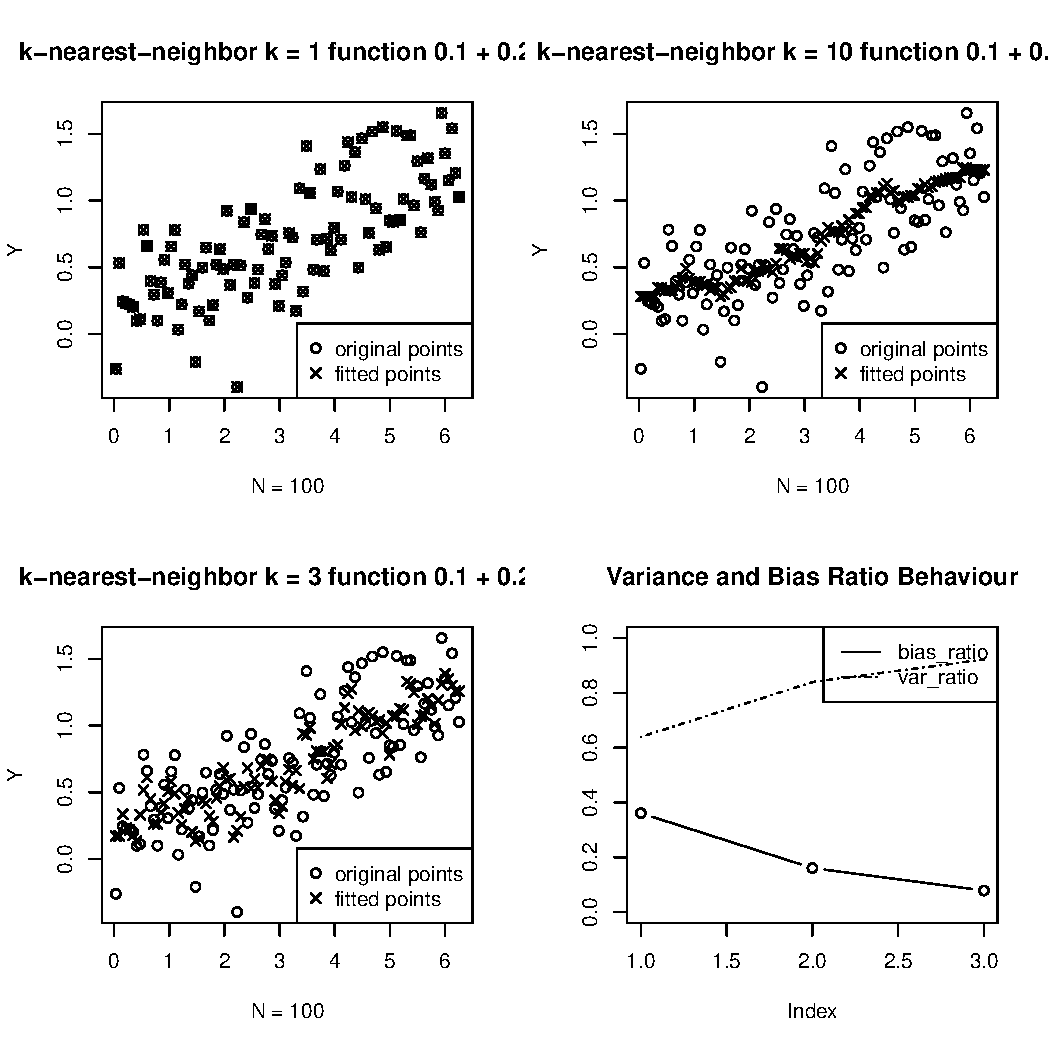
\includegraphics[width=\maxwidth]{figure/minimal-Haha} 
\begin{kframe}\begin{alltt}
\hlcom{# Fit a constant function(The same as fitting a knn with k = 100 since we only have ten}
\hlcom{# points in the trainning sample)}
\hlkwd{knn_model}\hlstd{(X_pre, X, Y,} \hlnum{100}\hlstd{)}
\end{alltt}
\begin{verbatim}
##   Mean_EPE var_ratio bias_ratio
## 1  0.02365    0.5391     0.4609
\end{verbatim}
\begin{alltt}
\hlcom{# Fit a linear model}
\hlstd{fit_linear} \hlkwb{<-} \hlkwd{lm}\hlstd{(Y} \hlopt{~} \hlstd{X)}
\hlstd{predict_linear} \hlkwb{<-} \hlstd{X_pre} \hlopt{*} \hlstd{fit_linear}\hlopt{$}\hlstd{coefficients[}\hlnum{2}\hlstd{]} \hlopt{+} \hlstd{fit_linear}\hlopt{$}\hlstd{coefficients[}\hlnum{1}\hlstd{]}
\hlstd{EPE_linear} \hlkwb{<-} \hlkwd{matrix}\hlstd{(}\hlnum{NA}\hlstd{,} \hlnum{1000}\hlstd{)}
\hlkwa{for} \hlstd{(i} \hlkwa{in} \hlnum{1}\hlopt{:}\hlnum{1000}\hlstd{) \{}
    \hlstd{EPE_linear[i]} \hlkwb{<-} \hlkwd{mean}\hlstd{((predict_linear[i]} \hlopt{-} \hlstd{Simu_Y[, i])}\hlopt{^}\hlnum{2}\hlstd{)}
\hlstd{\}}
\hlkwd{mean}\hlstd{(EPE_linear)}\hlopt{/}\hlstd{(}\hlnum{2} \hlopt{*} \hlstd{pi)}  \hlcom{# This is the estimated E(EPE(X)) under linear model}
\end{alltt}
\begin{verbatim}
## [1] 0.0147
\end{verbatim}
\begin{alltt}
\hlstd{Var_linear} \hlkwb{<-} \hlkwd{sum}\hlstd{((}\hlkwd{mean}\hlstd{(predict_linear)} \hlopt{-} \hlstd{predict_linear)}\hlopt{^}\hlnum{2}\hlstd{)}
\hlstd{Var_linear}
\end{alltt}
\begin{verbatim}
## [1] 108.7
\end{verbatim}
\begin{alltt}
\hlstd{Bias_linear} \hlkwb{<-} \hlkwd{sum}\hlstd{((}\hlkwd{colMeans}\hlstd{(Simu_Y)} \hlopt{-} \hlkwd{mean}\hlstd{(predict_linear))}\hlopt{^}\hlnum{2}\hlstd{)}
\hlkwd{sqrt}\hlstd{(Bias_linear)}
\end{alltt}
\begin{verbatim}
## [1] 11.49
\end{verbatim}
\begin{alltt}
\hlcom{# Fit a quadratic function}
\hlstd{fit_quadra} \hlkwb{<-} \hlkwd{lm}\hlstd{(Y} \hlopt{~} \hlstd{X} \hlopt{+} \hlkwd{I}\hlstd{(X}\hlopt{^}\hlnum{2}\hlstd{))}
\hlstd{predict_quadra} \hlkwb{<-} \hlstd{X_pre}\hlopt{^}\hlnum{2} \hlopt{*} \hlstd{fit_quadra}\hlopt{$}\hlstd{coefficients[}\hlnum{3}\hlstd{]} \hlopt{+} \hlstd{X_pre} \hlopt{*} \hlstd{fit_quadra}\hlopt{$}\hlstd{coefficients[}\hlnum{2}\hlstd{]} \hlopt{+}
    \hlstd{fit_quadra}\hlopt{$}\hlstd{coefficients[}\hlnum{1}\hlstd{]}
\hlstd{EPE_quadra} \hlkwb{<-} \hlkwd{matrix}\hlstd{(}\hlnum{NA}\hlstd{,} \hlnum{1000}\hlstd{)}
\hlkwa{for} \hlstd{(i} \hlkwa{in} \hlnum{1}\hlopt{:}\hlnum{1000}\hlstd{) \{}
    \hlstd{EPE_quadra[i]} \hlkwb{<-} \hlkwd{mean}\hlstd{((predict_quadra[i]} \hlopt{-} \hlstd{Simu_Y[, i])}\hlopt{^}\hlnum{2}\hlstd{)}
\hlstd{\}}
\hlkwd{mean}\hlstd{(EPE_quadra)}\hlopt{/}\hlstd{(}\hlnum{2} \hlopt{*} \hlstd{pi)}  \hlcom{# This is the estimated E(EPE(X)) under quadratic model}
\end{alltt}
\begin{verbatim}
## [1] 0.01481
\end{verbatim}
\begin{alltt}
\hlstd{Var_quadra} \hlkwb{<-} \hlkwd{sum}\hlstd{((}\hlkwd{mean}\hlstd{(predict_quadra)} \hlopt{-} \hlstd{predict_quadra)}\hlopt{^}\hlnum{2}\hlstd{)}
\hlstd{Var_quadra}
\end{alltt}
\begin{verbatim}
## [1] 109.5
\end{verbatim}
\begin{alltt}
\hlstd{Bias_quadra} \hlkwb{<-} \hlkwd{sum}\hlstd{((}\hlkwd{colMeans}\hlstd{(Simu_Y)} \hlopt{-} \hlkwd{mean}\hlstd{(predict_quadra))}\hlopt{^}\hlnum{2}\hlstd{)}
\hlkwd{sqrt}\hlstd{(Bias_quadra)}
\end{alltt}
\begin{verbatim}
## [1] 11.49
\end{verbatim}
\end{kframe}
\end{knitrout}



\end{document}
